\documentclass[letter,11pt]{article}

\usepackage[spanish,es-nodecimaldot]{babel}
\usepackage[utf8]{inputenc}

\usepackage{lmodern}
\usepackage[T1]{fontenc}
\usepackage{textcomp}

\usepackage[svgnames]{xcolor}
\colorlet{shadecolor}{Gainsboro!50}

\usepackage[labelfont=bf]{caption}
\usepackage{graphicx}
\usepackage{pstricks}

\usepackage{anysize}
\marginsize{3cm}{2cm}{2cm}{3cm}

\usepackage{url}
\usepackage{siunitx}
\usepackage{amsmath}
\usepackage{array}

\usepackage{caption}
\newcommand{\source}[1]{\vspace{-11pt} \caption*{\small{\textbf{Nota:} {#1}}}}

\usepackage{fancyhdr}
\usepackage{lastpage}
\pagestyle{fancy}
\fancyhf{}
\fancyhead[LE,RO]{Laboratorio de Física Básica II}
\fancyfoot[CO,CE]{\thepage\ de \pageref{LastPage}}

\special{papersize=215.9mm,279.4mm}

\usepackage[
    pdfauthor={Carlos Eduardo Caballero Burgoa},%
    pdftitle={Laboratorio de Física Básica II},%
    pdfsubject={Variación de la presión con la profundidad},%
    colorlinks,%
    citecolor=black,%
    filecolor=black,%
    linkcolor=black,%
    urlcolor=black,
    breaklinks]{hyperref}
\usepackage{breakurl}

\newcommand{\blankpage}{
\newpage
\thispagestyle{empty}
\mbox{}
\newpage
}

\renewcommand{\arraystretch}{1.2}

\title{Informe 5: Variación de la presión \\
con la profundidad}
\author{Carlos Eduardo Caballero Burgoa \\
    \small{\href{mailto:200201226@est.umss.edu}{200201226@est.umss.edu}}
}
\date{\today}

\begin{document}

\maketitle
\begin{center}
    \textbf{Grupo}: J2\\
    \textbf{Docente}: Ing. Milka Mónica Torrico Troche\\
    \textbf{Carrera}: Ing. Electromecánica
\end{center}

\begin{abstract}
Este documento detalla el experimento realizado en simulador para hallar la
relación funcional entre la presión y la profundidad en un fluido en reposo,
además del calculo de la densidad, para esto se realizó la medición de la
presión en un fluido a diferentes variaciones de profundidad; posteriormente se
calculó la relación funcional con el método de mínimos cuadrados, finalmente se
determinó el valor de la densidad, resultando ser:
$(1701.5 \pm 5.8)[kg/m^3]; 0.34\%$.
\end{abstract}

\section{Introducción}

Cuando un fluido (ya sea liquido o gaseoso) esta en reposo, este ejerce una
fuerza perpendicular a cualquier superficie, en contacto con este. Considerando
una superficie pequeña de área $dA$ centrada en un punto en el fluido; la
fuerza normal que el fluido ejerce sobre cada lado es $dF_{\perp}$. Se define
la \textbf{presión} ($P$) en ese punto como la fuerza normal por unidad de
área, es decir, la razón entre $dF_{\perp}$ y $dA$ \cite{Young&Freedman}.

\begin{equation}
    P = \frac{dF_{\perp}}{dA}
\label{presion}
\end{equation}
\vspace{0.10cm}

Es posible deducir una relación general entre la presión $P$ en cualquier
punto de un fluido de reposo y la profundidad $y$ del punto; si la densidad
$\rho$ tiene el mismo valor en todo el fluido (es decir, la densidad es
uniforme), al igual que la aceleración debida a la gravedad $g$.

\begin{figure}
\centering
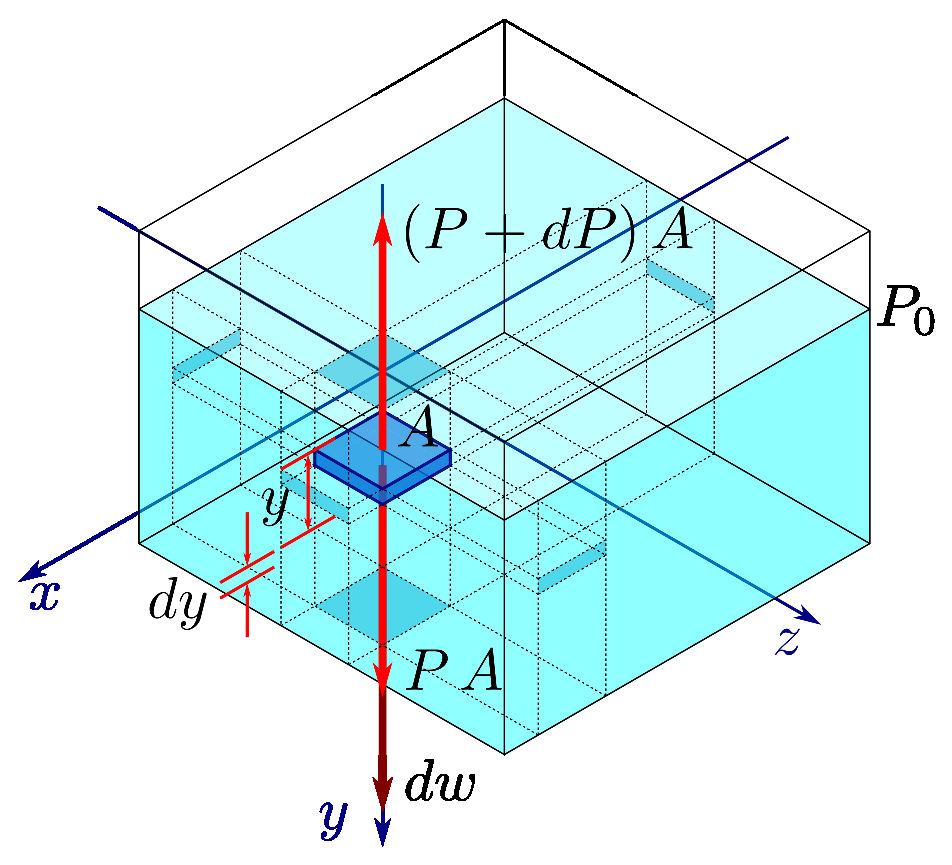
\includegraphics[width=0.50\textwidth]{resources/f1.eps}
\caption{Fuerzas sobre un elemento de fluido en equilibrio.}
\label{figura1}
\source{Física Universitaria Volumen I (p. 376), \\
Young, Hugh D. y Freedman, Roger A., 2013, Pearson.}
\end{figure}

Considerando un elemento de espesor $dy$, como puede verse en la
\textbf{Figura \ref{figura1}}; la superficie inferior y superior tiene un área
$A$, y están a distancias $y + dy$ y $y$ respectivamente.

El volumen ($dV$) del elemento es:

\begin{equation*}
    dV = A\,dy
\end{equation*}
\vspace{0.10cm}

Su masa ($dm$) y peso ($dw$) son:

\begin{equation*}
    dm = \rho\,dV = \rho\,A\,dy
\end{equation*}
\begin{equation}
    dw = dm\,g = \rho g\,A\,dy
\end{equation}
\vspace{0.10cm}

Considerando que las fuerzas que actúan sobre el elemento están en equilibrio,
tenemos:

\begin{equation*}
    \sum F_y = 0
\end{equation*}
\begin{equation*}
    P\,A - (P + dP)\,A + dw = 0
\end{equation*}
\begin{equation*}
    P\,A - (P + dP)\,A + \rho g\,A\,dy = 0
\end{equation*}
\begin{equation*}
    P\,A - P\,A - dP\,A + \rho g\,A\,dy = 0
\end{equation*}
\begin{equation*}
    - dP\,A + \rho g\,A\,dy = 0
\end{equation*}
\begin{equation*}
    - dP + \rho g\,dy = 0
\end{equation*}
\begin{equation*}
    dP = \rho g\,dy
\end{equation*}
\begin{equation}
    \frac{dP}{dy} = \rho g
\label{presion2}
\end{equation}
\vspace{0.10cm}

La \textbf{Ecuación \ref{presion2}} indica que si $y$ aumenta, $P$ aumenta.

Integrando la \textbf{Ecuación \ref{presion2}} desde la superficie hasta
el valor de profundidad $y$, resulta:

\begin{equation*}
    dP = \rho g\,dy
\end{equation*}
\begin{equation*}
    \int_{P_0}^{P} dP = \int_{0}^{h} \rho g\,dy
\end{equation*}
\begin{equation*}
    P\Biggr|_{P_0}^{P} = \rho g y\Biggr|_{0}^{h}
\end{equation*}
\begin{equation*}
    P - P_0 = \rho g h
\end{equation*}
\begin{equation}
    P = P_0 + \rho g h
\label{pascal}
\end{equation}
\vspace{0.10cm}

Por tanto, la presión es la misma en todos los puntos situados a una misma
profundidad, independiente de la forma del recipiente.

Para el experimento se verificará la \textbf{Ecuación \ref{pascal}}. A partir de
una profundidad establecida ($h$), se medirá la presión ($P$). Finalmente se
determinará el valor de la densidad ($\rho$) despejándola de la misma ecuación.

\section{Método experimental}

\begin{figure}
\centering
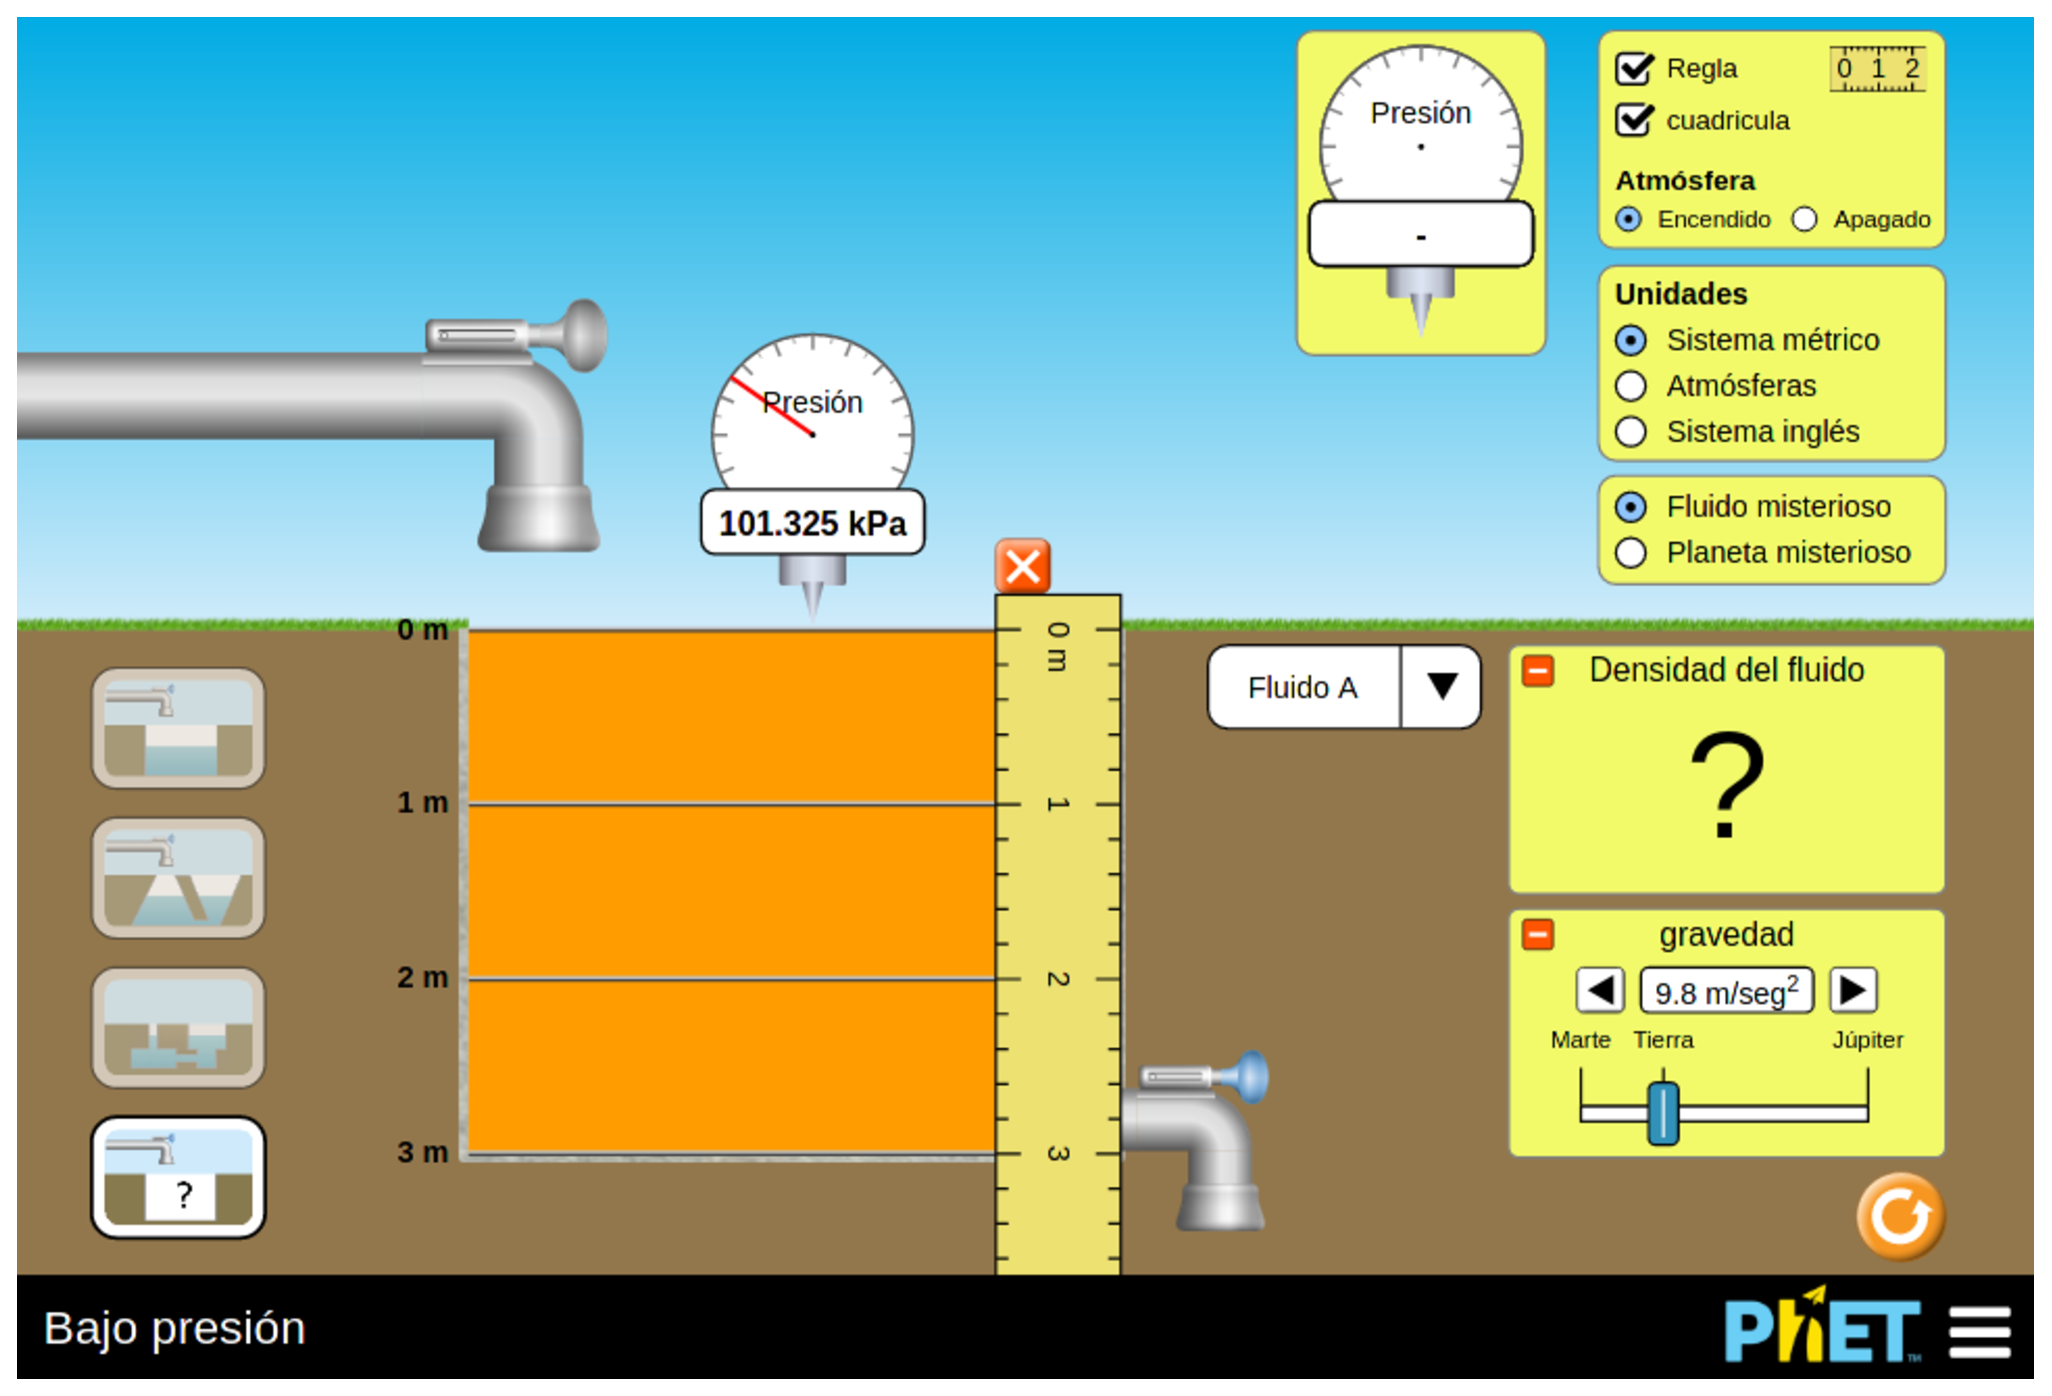
\includegraphics[width=0.90\textwidth]{resources/f2.eps}
\caption{Simulador de presión.}
\label{figura2}
\source{Fotografía propia.}
\end{figure}

Para la realización del experimento, se emplea el simulador \emph{PhET} «Bajo
presión», ubicado en la dirección web: \url{
https://phet.colorado.edu/sims/html/under-pressure/latest/under-pressure_es.html
}, tal como se presenta en la \textbf{Figura \ref{figura2}}.

Para el simulador, se registrarán diferentes valores de profundidad ($h$) para
medir su variación de presión ($P$).

Una vez medidos los datos, se procederá a graficar la relación profundidad vs.
presión del recipiente, y con la ayuda del método de los mínimos cuadrados, se
halla la relación funcional entre las variables.

Finalizando con el calculo del valor de la densidad ($\rho$), a partir de la
\textbf{Ecuación \ref{pascal}}:

\begin{equation*}
    B = \rho g
\end{equation*}
\vspace{0.10cm}

Despejando $\rho$, se obtiene:

\begin{equation}
    \rho = \frac{B}{g}
\label{densidad}
\end{equation}
\vspace{0.10cm}

\textbf{Datos necesarios para el experimento:} \\

Aceleración de la gravedad local:

\begin{equation*}
    g = (9.78 \pm 0.02)[m/s^2]
\end{equation*}
\vspace{0.10cm}

\textbf{Datos tomados en el experimento:} \\

En el \textbf{Cuadro \ref{cuadro1}}, se pueden ver los valores tomados del 
experimento, tanto la profundidad como la presión medida.

\begin{table}[!h]
\begin{center}
\begin{tabular}{|c||>{\centering}m{2.0cm}<{\centering}
                  |>{\centering}m{2.0cm}<{\centering}|
                |c||>{\centering}m{2.0cm}<{\centering}
                  |>{\centering}m{2.0cm}<{\centering}|}
\hline
$i$ & $h_i [m]$ & $P_i [kPa]$ & $i$ & $h_i [m]$ & $P_i [kPa]$
    \tabularnewline \hline \hline
 1 & 0.0 & 101.325 &  9 & 1.6 & 128.007 \tabularnewline \hline
 2 & 0.2 & 104.969 & 10 & 1.8 & 131.184 \tabularnewline \hline
 3 & 0.4 & 108.306 & 11 & 2.0 & 134.680 \tabularnewline \hline
 4 & 0.6 & 111.642 & 12 & 2.2 & 138.175 \tabularnewline \hline
 5 & 0.8 & 114.820 & 13 & 2.4 & 141.671 \tabularnewline \hline
 6 & 1.0 & 117.997 & 14 & 2.6 & 145.007 \tabularnewline \hline
 7 & 1.2 & 121.493 & 15 & 2.8 & 148.185 \tabularnewline \hline
 8 & 1.4 & 124.829 & 16 & 3.0 & 151.203 \tabularnewline \hline
\end{tabular}
\caption{Mediciones de presión en función de la profundidad.}
\label{cuadro1}
\source{Elaboración propia.}
\end{center}
\end{table}

\section{Resultados}

\begin{figure}
\centering
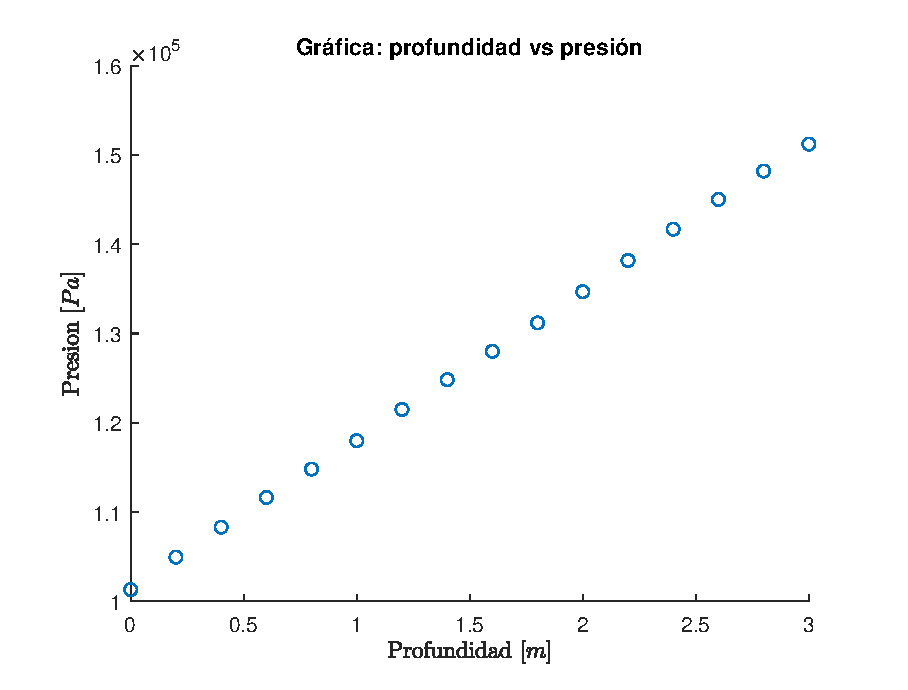
\includegraphics[width=0.80\textwidth]{resources/m1.eps}
\caption{Gráfica de longitud vs fuerza.}
\label{figura3}
\source{Elaboración propia.}
\end{figure}

A partir de los datos obtenidos se genera la gráfica de la
\textbf{Figura \ref{figura3}}.

Posteriormente se calculo la recta de mejor ajuste por el método de los mínimos
cuadrados, resultando los siguientes valores:

\begin{equation*}
    A = (101.51 \pm 0.08) [kPa]; 0.08\%
\end{equation*}
\begin{equation*}
    B = (16.64 \pm 0.04) [kPa/m]; 0.27\%
\end{equation*}
\vspace{0.10cm}

Siendo su coeficiente de correlación ($r$):

\begin{equation*}
    r = 0.9999
\end{equation*}
\vspace{0.10cm}

Considerando que el modelo de ajuste es:

\begin{equation*}
    P = A + B h
\end{equation*}
\vspace{0.10cm}

Por tanto la relación funcional entre $P$ y $h$, es:

\begin{equation*}
    P \propto h
\end{equation*}
\vspace{0.10cm}

Para el calculo de la densidad ($\rho$) se utiliza la
\textbf{Ecuación \ref{densidad}}, resultando:

\begin{equation*}
    \rho = (1701.5 \pm 5.8) [kg/m^3]; 0.34\%
\end{equation*}
\vspace{0.10cm}

\section{Conclusiones}

Se halló la relación funcional entre el incremento de la profundidad y
la presión, confirmándose la \textbf{Ecuación \ref{pascal}}.

También se calculó el valor de la densidad del fluido.

\begin{thebibliography}{99}

\bibitem{Young&Freedman} Young, Hugh D. y Freedman, Roger A. (2013).\\
Física Universitaria. Volumen 1.\\
13va Edición.\\
Capitulo 12.

\bibitem{GUIA} Departamento de Física - UMSS.\\
Laboratorio de Física Básica II.\\
Guía - Cartilla de laboratorio.\\
Gestión I/2020.

\end{thebibliography}

\newpage
\section*{Apéndice: Cálculos adicionales}

\subsection{Método de mínimos cuadrados}

Se calculan los parámetros de la recta por el método de los mínimos cuadrados,
con la ayuda de los datos presentados en el \textbf{Cuadro \ref{cuadro2}}.

\begin{table}[!h]
\begin{center}
\begin{tabular}{|c||>{\centering}m{1.8cm}<{\centering}
                  |>{\centering}m{1.8cm}<{\centering}
                  |>{\centering}m{1.8cm}<{\centering}|
                  |>{\centering}m{1.8cm}<{\centering}
                  |>{\centering}m{1.8cm}<{\centering}
                  |>{\centering}m{2.1cm}<{\centering}|}
\hline
$i$ & $x_i y_i\,(\num{e5})$ & $x^2_i$ & $y^2_i\,(\num{e10})$ &
    $Y_i\,(\num{e5})$ & $d_i$ & $d^2_i\,(\num{e4})$
    \tabularnewline \hline \hline
 1 &      0 &      0 & 1.0267 & 1.0151 & -182.6397 & 3.3357 \tabularnewline \hline
 2 & 0.2099 & 0.0400 & 1.1018 & 1.0484 &  133.2706 & 1.7761 \tabularnewline \hline
 3 & 0.4332 & 0.1600 & 1.1730 & 1.0816 &  142.1809 & 2.0215 \tabularnewline \hline
 4 & 0.6699 & 0.3600 & 1.2464 & 1.1149 &  150.0912 & 2.2527 \tabularnewline \hline
 5 & 0.9186 & 0.6400 & 1.3184 & 1.1482 &    0.0015 & 0.0000 \tabularnewline \hline
 6 & 1.1800 & 1.0000 & 1.3923 & 1.1815 & -151.0882 & 2.2828 \tabularnewline \hline
 7 & 1.4579 & 1.4400 & 1.4761 & 1.2148 &   16.8221 & 0.0283 \tabularnewline \hline
 8 & 1.7476 & 1.9600 & 1.5582 & 1.2480 &   24.7324 & 0.0612 \tabularnewline \hline
 9 & 2.0481 & 2.5600 & 1.6386 & 1.2813 & -125.3574 & 1.5714 \tabularnewline \hline
10 & 2.3613 & 3.2400 & 1.7209 & 1.3146 & -276.4471 & 7.6423 \tabularnewline \hline
11 & 2.6936 & 4.0000 & 1.8139 & 1.3479 & -108.5368 & 1.1780 \tabularnewline \hline
12 & 3.0398 & 4.8400 & 1.9092 & 1.3812 &   58.3735 & 0.3407 \tabularnewline \hline
13 & 3.4001 & 5.7600 & 2.0071 & 1.4144 &  226.2838 & 5.1204 \tabularnewline \hline
14 & 3.7702 & 6.7600 & 2.1027 & 1.4477 &  234.1941 & 5.4847 \tabularnewline \hline
15 & 4.1492 & 7.8400 & 2.1959 & 1.4810 &   84.1044 & 0.7074 \tabularnewline \hline
16 & 4.5361 & 9.0000 & 2.2862 & 1.5143 & -225.9853 & 5.1069 \tabularnewline \hline
\end{tabular}
\caption{Valores para el método de mínimos cuadrados.}
\label{cuadro2}
\source{Elaboración propia.}
\end{center}
\end{table}

\begin{equation*}
    n = 16
\end{equation*}
\begin{equation*}
    \sum x_i = 24
\end{equation*}
\begin{equation*}
    \sum y_i = 2023493
\end{equation*}
\begin{equation*}
    \sum x^2_i = 49.6000
\end{equation*}
\begin{equation*}
    \sum y^2_i = \num{2.5967e11}
\end{equation*}
\begin{equation*}
    \sum x_i y_i = \num{3.2615e6}
\end{equation*}
\begin{equation*}
    \Delta_1 = n \sum x^2_i - \left( \sum x_i \right)^2 = 217.6000
\end{equation*}
\begin{equation*}
    \Delta_2 = n \sum y^2_i - \left( \sum y_i \right)^2 = \num{6.0261e10}
\end{equation*}
\begin{equation*}
    A = \frac{\sum y_i \sum x^2_i - \sum x_i y_i \sum x_i}{\Delta_1} = \num{1.0151e5}
\end{equation*}
\begin{equation*}
    B = \frac{n \sum x_i y_i - \sum x_i \sum y_i}{\Delta_1} = \num{1.6640e4}
\end{equation*}
\begin{equation*}
    \sum d^2 = \num{3.8910e5}
\end{equation*}
\begin{equation*}
    \sigma^2 = \frac{\sum d^2_i}{n-2} = \num{2.7793e4}
\end{equation*}
\begin{equation*}
    \sigma_A = \sqrt{\frac{\sigma^2 \sum x^2_i}{\Delta_1}} = 79.5938
\end{equation*}
\begin{equation*}
    \sigma_B = \sqrt{\frac{\sigma^2 n}{\Delta_1}} = 45.2063
\end{equation*}
\vspace{0.10cm}

Parámetros de la recta obtenida:

\begin{equation*}
    A = (\num{1.0151e5} \pm 79.5938) [Pa]; 0.0784\%
\end{equation*}
\begin{equation*}
    B = (\num{1.6640e4} \pm 45.2063) [N/m]; 0.2717\%
\end{equation*}
\vspace{0.10cm}

Siendo el coeficiente de correlación:

\begin{equation*}
    R = \frac{n \sum x_i y_i - (\sum x_i)(\sum y_i)}{\sqrt{\Delta_1 \Delta_2}}
      = 0.9999
\end{equation*}
\vspace{0.10cm}

La ecuación de la recta resultante es:

\begin{equation*}
    y = \num{1.0151e5} + \num{1.6640e4}\,x
\end{equation*}
\vspace{0.10cm}

\subsection{Calculo de la densidad}

Para el calculo de la densidad, se utiliza la
\textbf{Ecuación \ref{densidad}}:

\begin{equation*}
    \rho = \frac{B}{g} = \frac{\num{1.6640e4}}{9.78} = \num{1.7015e3}
\end{equation*}
\vspace{0.10cm}

Y el error de la medición es:

\begin{equation*}
    \frac{\partial \rho}{\partial B} = \frac{1}{g}
\end{equation*}
\begin{equation*}
    \frac{\partial \rho}{\partial g} = -\frac{B}{g^2}
\end{equation*}
\begin{equation*}
    e_{\rho} = \sqrt{ \left(\frac{1}{g} \right)^2 e_B^2 + \left(-\frac{B}{g^2} \right)^2 e_g^2 } = \num{2.0910e-4}
\end{equation*}
\vspace{0.10cm}

Resultando:

\begin{equation*}
    \rho = (\num{1.7015e3} \pm \num{2.0910e-4}) [kg/m^3]; \num{1.2289e-5}\%
\end{equation*}
\vspace{0.10cm}

\end{document}

